\vspace{30px}\section{NTC thermistors}
Unlike the PTC thermistor, the negative-temperature-coefficient (NTC) thermistor behaves inversely. This semiconductor device experiences a decrease in resistivity as the temperature increases. Its exceptional sensitivity to temperature variations contributes to its popular use across various applications.
\todo{Make NTC introduction a little longer}





\subsection{Chrateristics}
The NTC thermistor and the PTC thermistor, even though their functioning is opposite, have the same characteristic equation. As aforementioned, the equation that describes the behavior of the resistance $R$ in relationship with the ambient temperature $T$ is the following \cite{Chen20091103}:

\begin{equation*}
    R = R_0 \, e^{\, \beta\left( \frac{1}{T} - \frac{1}{T_0}\right)}
\end{equation*}

\noindent Where $R$ is the resistance at temperature $T$, which should be measured in Kelvin degrees, and $R_0$ is the resistance value measured at operating temperature $T_0$. The $\beta$ coefficient describes the thermister constant which varies on temperature and materials used to build the device. It can be calculated using the same formula described in the PTC thermistors:

\begin{equation*}
    \beta = \frac{\ln{\frac{R_2}{R_1}}}{\frac{1}{T_2} - \frac{1}{T_1}}
\end{equation*}

\noindent By assuming that when $T_1 = 298.15 K = 25^\circ C$, $R_1 = 10k\Omega$ and when $T_2 = 358.15 K = 85^\circ C$. $R_2 = 1.4k\Omega$, it is possible to plot the resistance-temperature relationship of a negative temperature coefficient thermistor. As shown in figure \ref{fig:NTC_logarithmic}, the curve shows that as the temperature rises, the resistance value decreases respecting the aforementioned equation.

\begin{figure}[h]
    \centering
    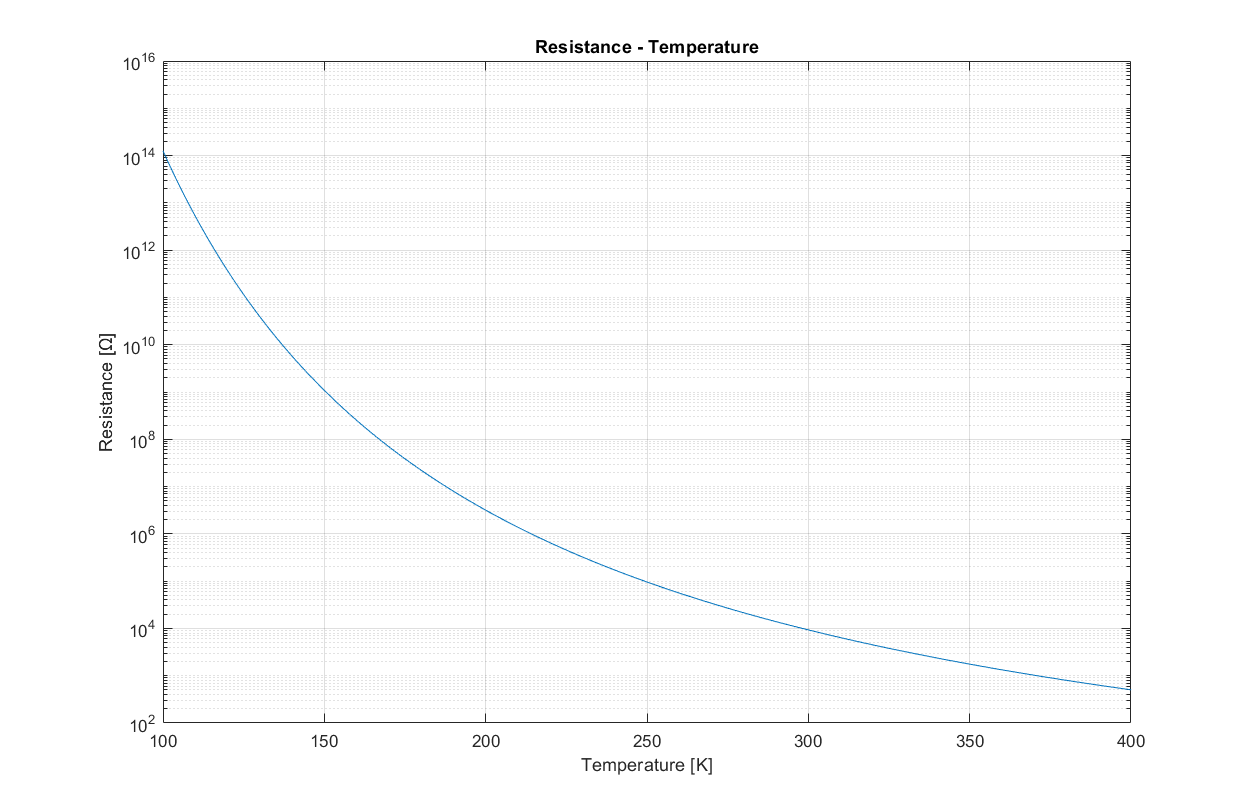
\includegraphics[width = .75\textwidth]{../res/plots/NTC_logarithmic.png}
    \caption{NTC resistance-temperature logarithmic curve, from -173°C to 326°C.}
    \label{fig:NTC_logarithmic}
\end{figure}

\FloatBarrier\noindent If the curve is restricted to more realistic temperature values (such as -13°C to 126°C), it's even more evident the inversely exponential curve which is described by the equation of the thermistor (figure \ref{fig:NTC_cartesian}).

\begin{figure}[h]
    \centering
    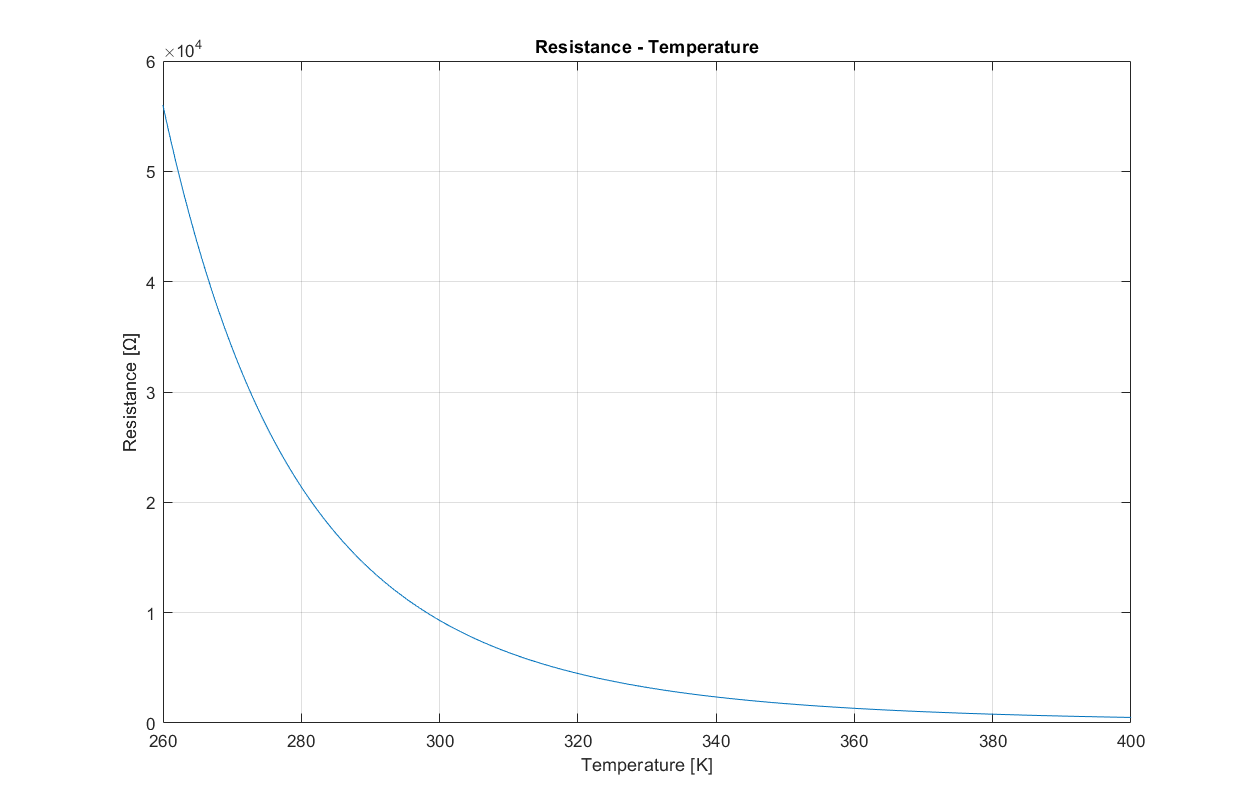
\includegraphics[width = .75\textwidth]{../res/plots/NTC_cartesian.png}
    \caption{NTC resistance-temperature curve, limited between -13°C and 126°C.}
    \label{fig:NTC_cartesian}
\end{figure}

\FloatBarrier\noindent By knowing the \textbf{dissipation constant} $\delta$ of the particular thermistor, it is possible to calculate the power consumption of the device, using the same equation mentioned on the PTC thermistor \cite{Jagtap201182}\cite{Keskin2005244}.

\begin{equation*}
    P = VI = \delta(T - T_0)
\end{equation*}

\noindent Where $T_0$ is the room temperature. Consequently, it is possible to calculate the equation for the voltage drop across the NTC thermistor and the current flowing through it \cite{Keskin2005244}.

\begin{equation*}
    V = (P\cdot R)^{\frac{1}{2}} \hspace{50px} I = \left(\frac{P}{R}\right)^{\frac{1}{2}}
\end{equation*}

\noindent By plotting the relationship between the current and the temperature, shown in figure \ref{fig:NTC_curr-temp}, it is evident that when the temperature increases, the current rises as well. This is a direct consequence of the fact that when the temperature rises the resistance of the thermistor is reduced and more current flows through the semiconductor device.

\begin{figure}[h]
    \centering
    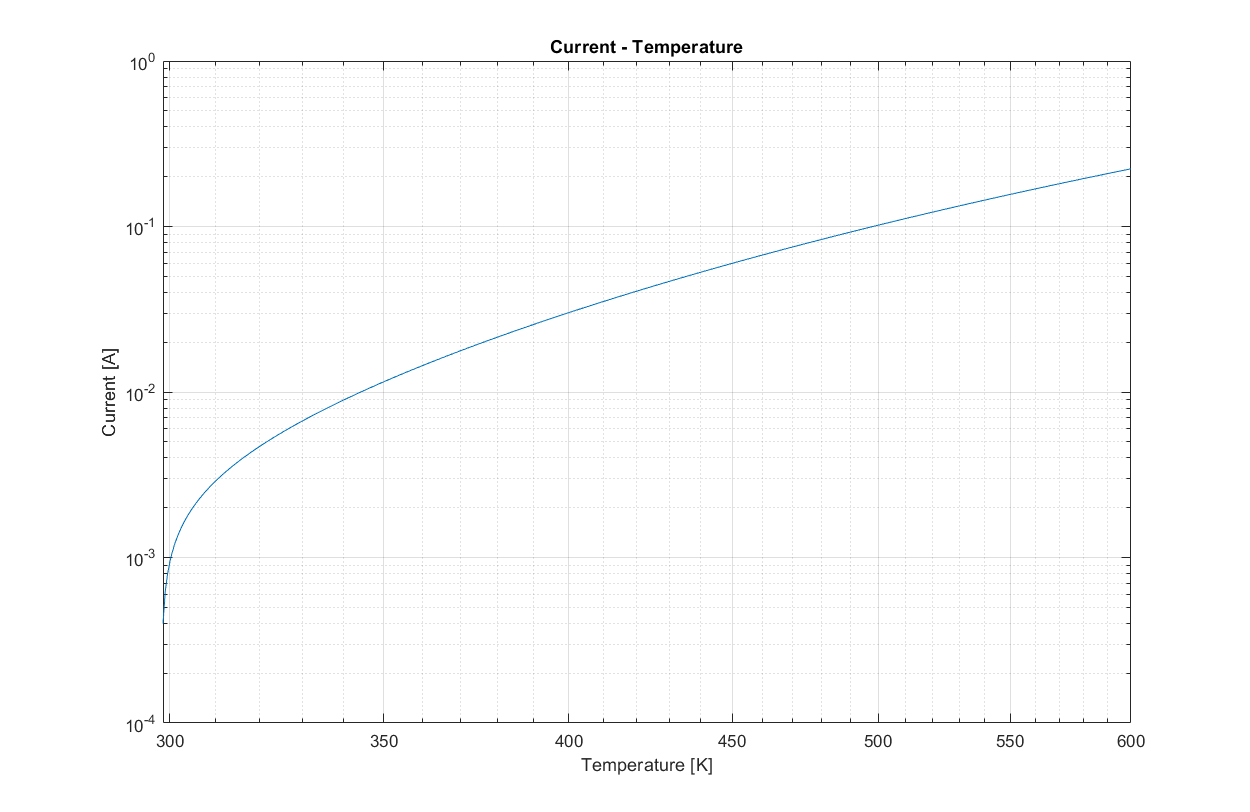
\includegraphics[width = .75\textwidth]{../res/plots/NTC_curr-temp.png}
    \caption{Corrent-temperature relationship of an NTC thermistor.}
    \label{fig:NTC_curr-temp}
\end{figure}

\FloatBarrier\noindent Observing the figure \ref{fig:NTC_volt-temp}, it is evident that the voltage-temperature decreases as the temperature increases. This phenomenon is attributed to the inverse relationship between temperature and resistance, leading to a corresponding decrease in the potential difference across the thermistor.

\begin{figure}[h]
    \centering
    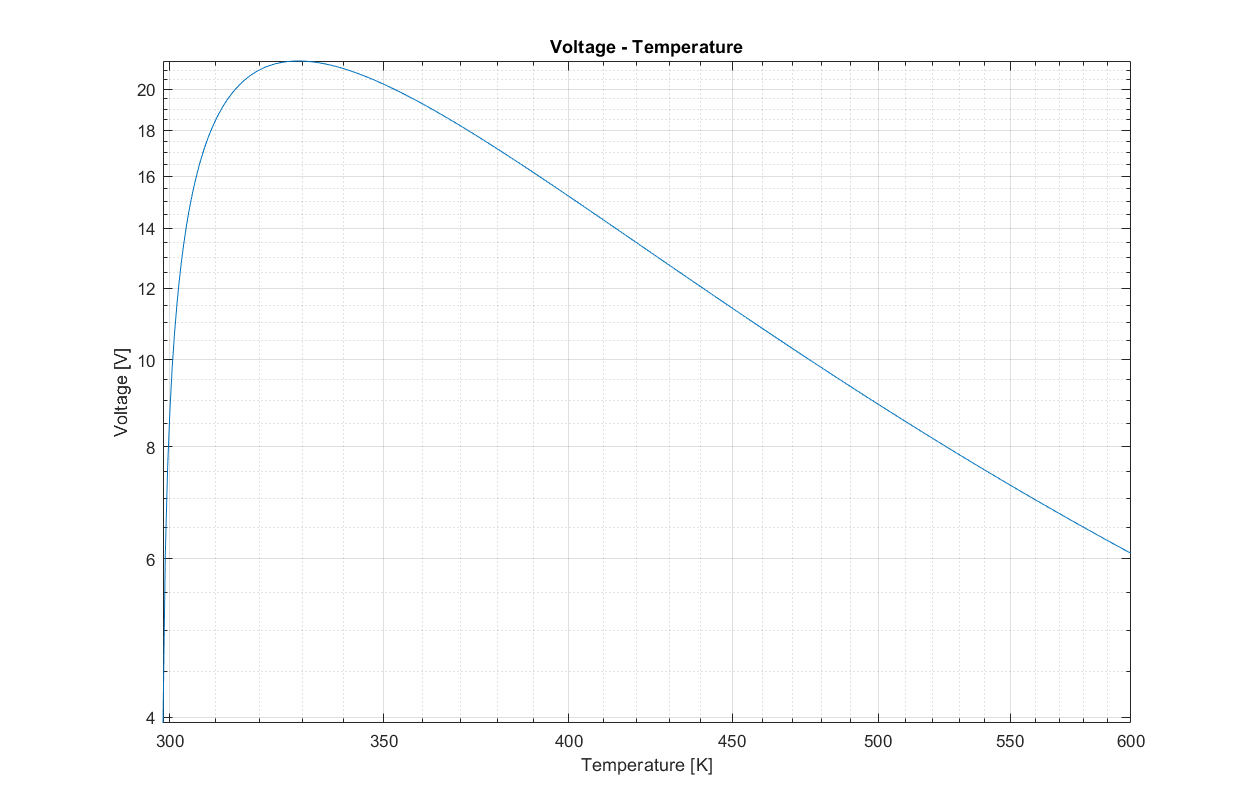
\includegraphics[width = .75\textwidth]{../res/plots/NTC_volt-temp.png}
    \caption{Voltage-temperature relationship of an NTC thermistor.}
    \label{fig:NTC_volt-temp}
\end{figure}

\FloatBarrier\noindent One of the most useful properties of an NTC thermistor is its VI characteristic curve, shown in the figure \ref{fig:NTC_curr-volt}. Noticeably, in the low-current region, there is low power dissipation and the thermistor does not heat up. In this state, the changes in the resistance will depend on the environment temperature rather than the heat produced by the device. When the current starts to rise it peaks at the maximum voltage level ($V_{max}$) and then the voltage starts to decrease due to the self-heating produced by the thermistor \cite{Jagtap201182}.

\begin{figure}[h]
    \centering
    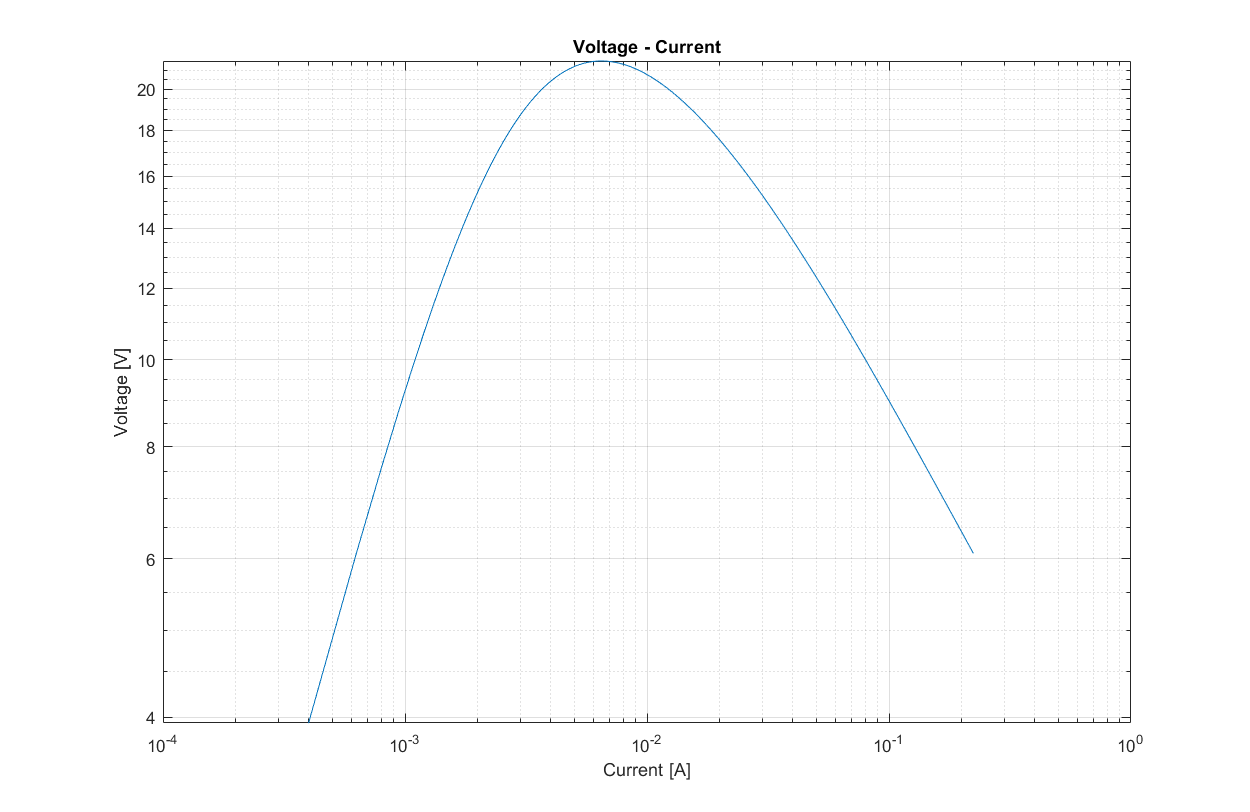
\includegraphics[width = .75\textwidth]{../res/plots/NTC_curr-volt.png}
    \caption{Voltage-current relationship of an NTC thermistor.}
    \label{fig:NTC_curr-volt}
\end{figure}


\FloatBarrier \subsection{Applications}
One of the most popular applications for the NTC thermistors is for \textit{temperature measurement} \cite{Chen20091103}\cite{Altenburg20011787}. This particular aspect of the negative temperature coefficient thermistor is vastly utilized in biomedical environments thanks to their high sensitivity to temperature oscillation \cite{Chen20091103}\cite{jones2010biomedical}. These devices are largely used in \textit{medical applications}, like the body-temperature measurement: this property can result in more advanced and sensitive thermometers or may be used for cancer reasearch and treatment \cite{Feteira2009967}.

A rather new application for the NTC thermistor takes into consideration its \textit{self-heating} property. When the thermistor is in a self-heat state its sensitivity to any external temperature variation is significantly high. This property can find applications to measure pressure, flow and composition of gasses \cite{Jagtap201182}.

Negative temperature coefficient thermistors are also used in \textit{home appliances} as far as washing machines, coffee makers, hair driers, fire alarms and home heating. Additionally, the NTC thermistors are used commonly in \textit{automobiles} to measure the temperature of the water and oil, the temperature of the cylinder and the braking system and the air-conditioning system \cite{Feteira2009967}.

Other interesting applications of these devices are for measuring the \textit{deep ocean} temperature \cite{Li2023} and for \textit{space applications} (like the PTC thermistors), specifically in the launch of the ETS-VI satellite and the H-II satellite \cite{Ishikawa1989116}.


